% !TeX root = ../../Book3.tex
% 纲要标题：## 第15章　正则序列与 Koszul 复形
% 纲要位置：工作记录/计划纲要.md，第 2444 行。
% 纲要细目（写作范围）：
% > 本编所需的复形、自由消解、链同伦与 Tor 在本章建立，Ext 与维数平移在后续章节建立；第四卷第6–9章（含第9.5节）给出这些工具的系统讨论。模论与范畴语言见预备知识总表；本编不以谱序列、导出范畴或 t-结构为前提。

\chapter{正则序列与 Koszul 复形}
\label{b3:ch:15}
\BookChapterNumber{b3:ch:15}

\begin{chapterabstract}
一个方程的乘法核可以用两项复形表示；几个方程的逐次正则性则由 Koszul 复形统一记录。本章先辨析模上非零因子、逐次商与末端非零的要求，证明局部环上有限生成模的正则序列可以重排，再从外代数写出 Koszul 微分、张量积符号及逐元加入的同调正合列。在此基础上证明正则序列的正合性，并对 Noether 局部环上的有限生成模证明逆命题。最后通过具体方程和 Tor 计算，比较独立方程、冗余关系、非约化结构与商环长度。
\end{chapterabstract}

\begin{learninggoals}
\begin{itemize}
\item 在每次取商后检验正则性，并说明局部性、有限性和末端非零条件的作用。
\item 写出低阶 Koszul 微分，核对张量积、外积和移位中的符号。
\item 用逐元加入的正合列证明正则性与 Koszul 同调消失之间的关系。
\item 区分自由消解与一般模上的正合 Koszul 复形，完成若干 Tor 的直接计算。
\end{itemize}
\end{learninggoals}

在交换环 \(R\) 中，一个元素 \(x\) 所决定的两项复形 \(0\to R\xrightarrow{\,x\,}R\to0\)，其末端商是 \(R/xR\)，起端同调却是 \(\operatorname{Ann}_R(x)\)。所以同一张乘法图同时记录“加上方程 \(x=0\)”与“\(x\) 是否为零因子”。若 \(k\) 为域，\(R=k[t]/(t^2)\)、\(x=\bar t\)，两端都有非零信息；仅写出商环并不能反映乘法的核。

\ProseParagraphBreak

多个方程可以把这些两项复形张量起来，得到 Koszul 复形。正则序列要求各方程在逐个取商后都保持非零因子的性质，且最后的商不能退化为零；这一条件将保证增广复形正合。这里的逐次独立性，是指每个 \(x_i\) 在 \(M/(x_1,\ldots,x_{i-1})M\) 上的乘法单射；它并不是参数的代数独立性，也不要求最后的商环约化或不可约。我们将从单个元素的核与像出发，追踪新添一个方程时同调如何变化。

\ProseParagraphBreak

本章使用\cref{b3:thm:nakayama,b3:thm:krull-intersection}，以及局部化、平坦基变换和第二卷第9章的外代数。复形、自由与投射消解、Ext、Tor 及维数平移的系统讨论安排在第四卷第6—9章；这里从自由模满射逐级构造消解，并通过链同伦说明 Tor 的定义不依赖消解的选择。

\ProseParagraphBreak
正则序列及 Koszul 复形可对照松村英之的《Commutative Ring Theory》\cite[\S16, pp. 123--129]{Matsumura1989CommutativeRingTheory}，其中 Theorems 16.4--16.5 分别给出逐元加入的同调正合列与正合性判据。本章把这些映射和符号逐项写出；一元情形应当始终作为核对一般公式的基准。

% 纲要内容（仅作写作计划，尚非教材正文）：
%
% > 本编所需的复形、自由消解、链同伦与 Tor 在本章建立，Ext 与维数平移在后续章节建立；第四卷第6–9章（含第9.5节）给出这些工具的系统讨论。模论与范畴语言见预备知识总表；本编不以谱序列、导出范畴或 t-结构为前提。
%

% !TeX root = ../../Book3.tex
% 纲要标题：### 15.1 正则序列
% 纲要位置：工作记录/计划纲要.md，第 2448 行。
% 纲要细目（写作范围）：
% * 模上非零因子及逐次商
% * 正则序列的次序问题
% * 平坦基变换、忠实平坦反映与局部化；区分逐次单射和末端商非零
% * 局部环上有限生成模的基本版本固定 \(M\ne0\)、各元素在极大理想中以及末端商非零的约定；零模的深度约定另列，避免定义间的退化冲突

\section{正则序列}
\label{b3:sec:1501}

依次施加几个方程时，每一步都可能产生新的零化关系，因此不能只在原模上逐个检查元素。正则序列要求在每个逐次商上重新检验乘法单射，并保留非零的最终商。


% 纲要内容（仅作写作计划，尚非教材正文）：
%
% * 模上非零因子及逐次商
% * 正则序列的次序问题
% * 平坦基变换、忠实平坦反映与局部化；区分逐次单射和末端商非零
% * 局部环上有限生成模的基本版本固定 \(M\ne0\)、各元素在极大理想中以及末端商非零的约定；零模的深度约定另列，避免定义间的退化冲突
%

\subsection{模上非零因子与逐次商}
\label{b3:subsec:1501:01}

一个方程对模的影响，要同时考察它删去了什么和留下了什么。乘法 \(m\mapsto xm\) 若有核，方程 \(x=0\) 已在原模中遇到被 \(x\) 零化的部分；若其商为零，则这个方程把整个模都消去了。正则序列排除这两种情形，并要求每增加一个方程后重新作同样的检查。

\begin{definition}\label{b3:def:regular-sequence}
设 \(R\) 为交换环，\(M\ne0\) 为 \(R\) 模。给定 \(x\in R\)，若乘法映射 \(M\xrightarrow{x}M\) 单射，则称 \(x\) 为 \(M\) 上的\term[mo-feilingyinzi]{非零因子}[non-zero-divisor on a module]。设 \(r\ge0\) 为整数，\(x_1,\ldots,x_r\in R\)，记
\[
M_i=M/(x_1,\ldots,x_i)M,\qquad M_0=M.
\]
若每个 \(x_i:M_{i-1}\rightarrow M_{i-1}\) 都单射，且 \(M_r\ne0\)，则称有序组 \(x_1,\ldots,x_r\) 为一个 \(M\) 上的\term[zhengze-xulie]{正则序列}[regular sequence on a module]。取 \(M=R\) 时称为 \(R\) 的正则序列。空序列在非零模上正则。
\end{definition}

末端商非零也保证每个中间商非零，因为末端商是它们的商。特别地，单元素序列 \((x)\) 在非零模 \(M\) 上正则，当且仅当乘 \(x\) 单射且 \(xM\ne M\)。非零因子只满足前一个条件；单位元的乘法是双射，所以它是非零因子，却会使 \(M/xM=0\)，不能成为正则序列的第一项。对 \(R=k[X,Y]\)，序列 \(X,Y\) 正则：第一次商是 \(k[Y]\)，其中 \(Y\) 的乘法单射，最后的商为 \(k\ne0\)。序列 \(X,XY\) 则不正则，因为 \(XY\) 在 \(R/(X)\) 中为零。

\ProseParagraphBreak
模也会改变结论。同一个 \(X\in k[X,Y]\) 在环本身上是非零因子，在模 \(k[X,Y]/(X)\) 上却把所有元素送到零。此后说“正则”时必须说明所作用的模，不能只看生成理想的表达式。

\subsection{正则序列的次序}
\label{b3:subsec:1501:02}

逐次取商使次序看起来不可避免。对一般环与模，次序确实可能改变正则性。例如令
\[
R=k[X,Y],\qquad M=R\oplus R/(X-1,Y).
\]
在第二个直和项上，\(X\) 作用为恒等映射，\(Y\) 作用为零。因此 \(X\) 在 \(M\) 上单射，且 \(M/XM\cong k[Y]\)，所以 \(X,Y\) 是 \(M\) 正则序列；但 \(Y\) 在 \(M\) 上已有非零核，\(Y,X\) 不是正则序列。取商 \(M/XM\) 时，第二个直和项被完全消去，后续的 \(Y\) 便看不到这个直和项中原有的零化关系。先施加 \(Y\) 则会立即遇到这些关系。

\begin{theorem}\label{b3:thm:regular-sequence-permutation}
设 \((R,\mathfrak m)\) 为交换 Noether 局部环，\(M\ne0\) 为有限生成的 \(R\) 模。若 \(x_1,\ldots,x_r\in\mathfrak m\) 是 \(M\) 正则序列，则其任意置换仍为 \(M\) 正则序列。
\end{theorem}
\begin{proof}
任意置换可分解为相邻交换，只需在已经除去前面各项后的非零有限生成模 \(N\) 上交换相邻的 \(x,y\)。已知 \(x\) 在 \(N\) 上单射，\(y\) 在 \(N/xN\) 上单射；交换后要分别证明 \(y\) 在 \(N\) 上单射，以及 \(x\) 在 \(N/yN\) 上单射。

若 \(yn=0\)，在 \(N/xN\) 中的单射性先给出 \(n=xn_1\)；由 \(xyn_1=0\) 和 \(x\) 单射得 \(yn_1=0\)。因此同一个论证还能对 \(n_1\) 使用，反复进行得到 \(n\in x^aN\) 对每个 \(a\ge0\) 成立。这里需要排除一个非零元素被任意高次的 \(x\) 整除。环 \(R\) 为 Noether 环、\(N\) 有限生成，且 \((x)\subseteq\mathfrak m=J(R)\)，所以\cref{b3:thm:krull-intersection}给出 \(\bigcap_{a\ge0}x^aN=0\)，从而 \(n=0\)。故 \(y\) 在 \(N\) 上单射。

若 \(xn=yn'\)，则在 \(N/xN\) 中有 \(y\bar n'=0\)，所以 \(n'=xn''\)。代回并约去 \(x\)，得到 \(n=yn''\)。这证明 \(x\) 在 \(N/yN\) 上单射。两个次序的末端商同为 \(N/(x,y)N\)，保持非零，后续逐次商也相同。因此相邻交换保持正则性。
\end{proof}

这里 Noether 性和有限性用于 Krull 交定理，元素位于极大理想中则排除了前例中单位元提前消去一部分模的现象。不能把这些假设从结论中删掉。

\subsection{平坦基变换与局部化}
\label{b3:subsec:1501:03}

\begin{proposition}\label{b3:prop:regular-sequence-base-change}
设 \(R\rightarrow S\) 为交换环之间的平坦同态，\(M\ne0\) 为 \(R\) 模，\(x_1,\ldots,x_r\) 为 \(M\) 正则序列。若
\[
\bigl(M/(x_1,\ldots,x_r)M\bigr)\otimes_RS\ne0,
\]
则其像为 \(M\otimes_RS\) 上的正则序列。特别地，忠实平坦扩张保持并反映正则序列。
\end{proposition}
\begin{proof}
每一步的短正合列 \(0\rightarrow M_{i-1}\xrightarrow{x_i}M_{i-1}\rightarrow M_i\rightarrow0\) 经平坦张量后仍正合，而余核为相应的逐次商。因此平坦性自动保持所有逐次乘法的单射性，却不保证非零的末端商在张量后仍非零；命题的附加条件正是保证这一点。末端商是 \(M\otimes_RS\) 的商，所以该条件也保证起始模非零。若同态忠实平坦，则非零模的张量仍非零，这个条件自动满足。

反过来，设扩张后的序列正则；平坦性使每个乘法核的张量积等于变基后乘法的核，因而这些张量积为零。忠实性再给出原核为零。原末端商若为零，其张量也将为零，与变基后的正则性矛盾，故原序列正则。
\end{proof}

因此局部化保持逐步单射；但末端商可能消失。设 \(R\) 为交换 Noether 环，\(M\ne0\) 为有限生成的 \(R\) 模，\(x_1,\ldots,x_r\) 为 \(M\) 正则序列，\(I=(x_1,\ldots,x_r)\)。在 \(\mathfrak p\in\operatorname{Supp}M\cap V(I)\) 处，\(M_{\mathfrak p}\) 是非零有限生成模，且 \(IR_{\mathfrak p}\subseteq\mathfrak pR_{\mathfrak p}\)；\cref{b3:thm:nakayama}保证 \(M_{\mathfrak p}/IM_{\mathfrak p}\ne0\)，故序列的像仍正则。在不包含 \(I\) 的素理想处，某个 \(x_i\) 成为单位，末端商则为零。

\ProseParagraphBreak
反向只检查 \(\operatorname{Supp}M\cap V(I)\) 则可能漏掉原来的乘法核。回到 \(R=k[X,Y]\)、\(M=R\oplus R/(X-1,Y)\)，取 \(I=(X,Y)\)。唯一包含 \(I\) 的素理想是 \(\mathfrak m=(X,Y)\)；在这里 \(X-1\) 为单位，第二个直和项的局部化为零，所以 \(M_{\mathfrak m}\cong R_{\mathfrak m}\)。序列 \(Y,X\) 在这个局部模上正则，因为除去 \(Y\) 后得到 \(k[X]_{(X)}\)，再除去 \(X\) 后得到 \(k\)。但原模中乘 \(Y\) 的核正是被局部化删去的第二个直和项，它支撑在 \((X-1,Y)\)，这个点不属于 \(V(I)\)。若要检验原来每个乘法的单射性，应在原环的全部极大理想处检验其核，而不是只检验末端商的支集。

\subsection{局部环上有限生成模的正则序列：非退化约定}
\label{b3:subsec:1501:04}

此后局部理论的基本对象固定为 Noether 局部环 \((R,\mathfrak m)\) 上的非零有限生成模 \(M\)，并只从 \(\mathfrak m\) 中选取正则序列。每个有限生成商模 \(M_i\) 若由非零的 \(M_{i-1}\) 除以 \(x_iM_{i-1}\) 得到，Nakayama 引理保证它仍非零。因此在这一范围内，检查逐次乘法单射已经足够；定义中的末端非零条件仍保留，以便在其他情形中准确使用。

\ProseParagraphBreak
对零模，所有乘法映射都单射；若允许以此构成任意长正则序列，长度便不再反映非零模上逐次正则性的限制。本书不在零模上定义上述非退化正则序列；下一章另外约定 \(\operatorname{depth}_R0=+\infty\)，使短正合列中的深度公式统一成立。这个数值约定不改变本章的定义。

% !TeX root = ../../Book3.tex
% 纲要标题：### 15.2 Koszul 复形
% 纲要位置：工作记录/计划纲要.md，第 2455 行。
% 纲要细目（写作范围）：
% * 外代数上的 Koszul 微分
% * 一元情形与张量积构造
% * 符号约定、微分平方为零与乘法同伦；同调的局部化和支集、含单位理想时的退化
% * 生成元可逆线性变换诱导的 Koszul 复形同构

\section{Koszul 复形}
\label{b3:sec:1502}

一条乘法映射记录一个方程的核与商，多个方程则还需要记录它们之间的关系。外代数的符号使这些关系组成复形，其同调能同时反映不同阶的失效。


% 纲要内容（仅作写作计划，尚非教材正文）：
%
% * 外代数上的 Koszul 微分
% * 一元情形与张量积构造
% * 符号约定及微分平方为零
% * 生成元可逆线性变换诱导的 Koszul 复形同构
%

\subsection{外代数上的 Koszul 微分}
\label{b3:subsec:1502:01}

\begin{definition}\label{b3:def:koszul-complex}
设 \(R\) 为交换环，\(r\) 为非负整数，\(x=(x_1,\ldots,x_r)\in R^r\)，令 \(F=R^r\) 的标准基为 \(e_1,\ldots,e_r\)。取
\[
K_i(x;R)=\bigwedge^i_RF\quad(0\le i\le r),\qquad K_i=0\quad(i<0\;\text{或}\;i>r),
\]
并以 \(R\) 线性延拓规定
\begin{equation}\label{b3:eq:koszul-differential}
\mathrm{d}_i(e_{j_1}\wedge\cdots\wedge e_{j_i})
=\sum_{a=1}^i(-1)^{a-1}x_{j_a}
e_{j_1}\wedge\cdots\wedge\widehat e_{j_a}\wedge\cdots\wedge e_{j_i}.
\end{equation}
这里 \(j_1<\cdots<j_i\)，帽号表示删去该因子，\(\mathrm{d}_0=0\)。所得链复形记为 \(K_\bullet(x;R)\)，称为 \(x\) 的\term[koszul-fuxing]{Koszul 复形}[Koszul complex]。对 \(R\) 模 \(M\)，定义 \(K_\bullet(x;M)=K_\bullet(x;R)\otimes_RM\)。
\end{definition}
\symidx{\(K_\bullet(x;M)\)：Koszul 复形}

设 \(R\) 为交换环，\(C_\bullet\) 为 \(R\) 模的链复形。本章采用下标递降的微分 \(\mathrm{d}_i:C_i\rightarrow C_{i-1}\)，它满足 \(\mathrm{d}_{i-1}\mathrm{d}_i=0\)。核 \(Z_i=\ker \mathrm{d}_i\) 中的元素称为\term[quan]{圈}[cycle]，像 \(B_i=\operatorname{im}\mathrm{d}_{i+1}\) 中的元素称为\term[bianjie]{边界}[boundary]。微分的复合为零保证 \(B_i\subseteq Z_i\)，其商 \(H_i(C)=Z_i/B_i\) 为\term[tongdiao-mo]{同调模}[homology module]；它记录核中还有哪些元素不能由前一级的像解释。这与第四卷的上链记号 \(C^{-i}=C_i\) 相容；上链微分仍升次。本节先把所需链复形直接写出，微分平方为零将在下文核验。

对任意 \(R\) 模 \(M\)，Koszul 复形的次数一到次数零的映射为
\[
M^r\xrightarrow{(x_1\ \cdots\ x_r)}M.
\]
它的像是 \(IM\)，其中 \(I=(x_1,\ldots,x_r)\)，而次数零的微分为零，故总有
\[
H_0(x;M)=M/IM.
\]
这个零次同调就是施加全部方程后所得的商；正次数同调则记录 Koszul 复形在相应次数未能正合的部分。

\ProseParagraphBreak
比较两个复形时，各次数的映射还须尊重微分，才能把关于核与像的比较传到同调。具体地，设 \(R\) 为交换环，\(C_\bullet,D_\bullet\) 为 \(R\) 模的链复形。若一族 \(R\) 线性映射 \(f_i:C_i\to D_i\) 满足 \(\mathrm{d}_Df_i=f_{i-1}\mathrm{d}_C\)，则称 \(f=(f_i)\) 为从 \(C_\bullet\) 到 \(D_\bullet\) 的\term[lian-yingshe]{链映射}[chain map]。对圈 \(z\)，相容式给出 \(\mathrm{d}_Df_i(z)=0\)；对边界 \(\mathrm{d}_Cw\)，它给出 \(f_i(\mathrm{d}_Cw)=\mathrm{d}_Df_{i+1}(w)\)。所以圈映到圈、边界映到边界，从而诱导同调模之间的同态。

\subsection{一元情形与张量积构造}
\label{b3:subsec:1502:02}

一元情形为
\[
K_\bullet(x;M):\qquad 0\longrightarrow M\xrightarrow{x}M\longrightarrow0,
\]
左边的 \(M\) 位于次数一，右边位于次数零。因此
\[
H_1(x;M)=0:_Mx,\qquad H_0(x;M)=M/xM.
\]
二元情形的全部矩阵则是
\[
0\longrightarrow M\xrightarrow{\binom{-y}{x}}M^2
\xrightarrow{(x\ \ y)}M\longrightarrow0.
\]
首个矩阵来自 \(\mathrm{d}(e_1\wedge e_2)=xe_2-ye_1\)。两个矩阵的复合把 \(c\in M\) 送到 \(x(-yc)+y(xc)=0\)，所以二元情形的微分平方为零正是交换律的结果。次数一的圈是满足 \(xa+yb=0\) 的关系 \((a,b)\)，边界则是 \((-yc,xc)\) 这种由交换律直接产生的 Koszul 关系。因此
\[
H_1(x,y;M)
=\frac{\{(a,b)\in M^2:xa+yb=0\}}
       {\{(-yc,xc):c\in M\}},
\]
它保留不能由这些 Koszul 关系得到的其余关系。

把每个方程的两项复形一起张量，就得到多元 Koszul 复形。下面的符号约定保证张量微分与外积微分相容。

\begin{proposition}\label{b3:prop:koszul-tensor}
设 \(R\) 为交换环，\(r\) 为非负整数，\(x_1,\ldots,x_r\in R\)。约定任意两个 \(R\) 模链复形 \(C_\bullet,D_\bullet\) 的张量积在次数 \(n\) 取 \(\bigoplus_{p+q=n}C_p\otimes_RD_q\)，并对齐次元 \(u\in C_p,v\in D_q\) 规定
\[
\mathrm{d}(u\otimes v)=\mathrm{d}_Cu\otimes v+(-1)^p u\otimes \mathrm{d}_Dv,
\]
在此约定下有链复形同构
\[
K_\bullet(x_1,\ldots,x_r;R)
\cong K_\bullet(x_1;R)\otimes_R\cdots\otimes_RK_\bullet(x_r;R).
\]
\end{proposition}
\begin{proof}
上述张量微分连续作用两次时，\(\mathrm{d}_C^2\) 与 \(\mathrm{d}_D^2\) 所给的项为零，两个交叉项的符号分别为 \((-1)^{p-1}\) 与 \((-1)^p\)，相加也为零，因而它确实定义链复形。在二元情形中，\(e_1\otimes e_2\) 的第一个因子次数为一，所以
\[
\mathrm{d}(e_1\otimes e_2)
=x_1(1\otimes e_2)-x_2(e_1\otimes1),
\]
恰好对应 \(\mathrm{d}(e_1\wedge e_2)=x_1e_2-x_2e_1\)。一般地，在右边每个因子中选择次数零的 \(1\) 或次数一的 \(e_j\)。恰有 \(i\) 个次数一因子的张量给出次数 \(i\) 的一组基，按指标顺序送到相应外积。在第 \(a\) 个次数一因子上作用微分时，前面有 \(a-1\) 个次数一因子，张量微分的符号为 \((-1)^{a-1}\)，与\eqref{b3:eq:koszul-differential}一致。这给出各次数的双射并保持微分；\(r=0\) 时两边均为集中在次数零的 \(R\)。
\end{proof}

\subsection{符号约定与微分平方为零}
\label{b3:subsec:1502:03}

\begin{proposition}\label{b3:prop:koszul-signs-homotopy}
设 \(R\) 为交换环，\(r\) 为非负整数，\(x=(x_1,\ldots,x_r)\in R^r\)，\(M\) 为 \(R\) 模，\(I=(x_1,\ldots,x_r)\)。Koszul 微分满足 \(\mathrm{d}^2=0\)，并且 \(I\) 零化每个 \(H_i(x;M)\)。对每个整数 \(i\) 和每个含一的乘法集 \(S\subseteq R\)，有自然同构
\[
S^{-1}H_i(x;M)\cong H_i(x/1;S^{-1}M),
\]
其中右端在 \(S^{-1}R\) 上计算，\(x/1=(x_1/1,\ldots,x_r/1)\)。此外，
\[
\operatorname{Supp}_R H_i(x;M)
\subseteq\operatorname{Supp}_R M\cap V(I).
\]
若 \(I=R\)，则所有 \(H_i(x;M)\) 都为零；当 \(M\ne0\) 时，这样的序列不满足本书正则序列的约定。
\end{proposition}
\begin{proof}
二元计算中的两种次序在一般情形中也逐对出现。在一次外积上连续删去第 \(a\) 与第 \(b\) 个因子，其中 \(a<b\)，两种删法分别带符号
\[
(-1)^{a-1+b-2},\qquad (-1)^{b-1+a-1}.
\]
两项的系数同为 \(x_{j_a}x_{j_b}\)，符号相反，所以逐对相消。此论证在特征二也成立，因为此时两项之和为零。

令 \(h_j(w)=e_j\wedge w\)，并张量上 \(M\) 的恒等映射，得到次数升一的映射 \(h_j\)。外积微分满足 \(\mathrm{d}(e_j\wedge w)=x_jw-e_j\wedge\mathrm{d}w\)，移项便得
\[
\mathrm{d} h_j+h_j\mathrm{d}=x_j\operatorname{id}.
\]
若 \(\mathrm{d}w=0\)，便有 \(x_jw=\mathrm{d}(h_jw)\)，即 \(x_j\) 乘一个圈得到边界。因此 \(x_jH_i=0\)，任意 \(I\) 中元素也零化同调。

在外幂的标准基下，每个 \(K_i(x;M)\) 是有限个 \(M\) 的直和。这些外积基向量及微分公式经局部化，分别给出 \(K_i(x/1;S^{-1}M)\) 及其微分。由\cref{b3:thm:localization-exact}，局部化与微分的核、像和商相容，所以圈模与边界模局部化后仍是相应的圈模与边界模，再取商就得到所述同调同构。若 \(M_{\mathfrak p}=0\)，局部化后的复形各项都为零，故同调也为零。若 \(\mathfrak p\notin V(I)\)，某个 \(x_j/1\) 在 \(R_{\mathfrak p}\) 中可逆，又零化局部化后的同调，该同调只能为零。这证明支集包含于 \(\operatorname{Supp}_R M\cap V(I)\)，不需要有限生成假设。

若 \(1=\sum_j a_jx_j\)，取 \(h=\sum_j a_jh_j\)，则 \(\mathrm{d}h+h\mathrm{d}=\operatorname{id}\)。对任意圈 \(w\)，这个等式给出 \(w=\mathrm{d}(hw)\)，所以全部同调为零，包括 \(H_0=M/IM\)。但末端商为零，故在 \(M\ne0\) 时不能据此得到正则序列。例如，对域 \(k\)，在 \(A=k[X,Y]_{(X)}\) 中，\(Y\) 因为不属于 \((X)\) 而成为单位。因此 \(K_\bullet(X,Y;A)\) 的全部同调消失，而非零环 \(A\) 的末端商 \(A/(X,Y)A\) 为零，序列 \(X,Y\) 不正则。
\end{proof}

设 \(C_\bullet,D_\bullet\) 为交换环 \(R\) 上的链复形，\(f,g:C_\bullet\rightarrow D_\bullet\) 为链映射。若存在 \(R\) 线性映射 \(h_i:C_i\rightarrow D_{i+1}\)，使 \(f-g=\mathrm{d}_Dh+h\mathrm{d}_C\)，则称 \(f\) 与 \(g\) \term[lian-tonglun]{链同伦}[chain homotopy]。上面构造的 \(h_j\) 表明乘法 \(x_j\) 与零映射链同伦。链同伦映射在同调上相同：对圈 \(z\)，有 \((f-g)z=\mathrm{d}_D(hz)\)。

\ProseParagraphBreak
生成元的重排是可逆线性变换的一种特例。添加另一个生成元的倍数或用单位倍替换一个生成元，也有同样的复形不变性。

\begin{proposition}[生成元的可逆线性变换]\label{b3:prop:koszul-generator-change}
设 \(R\) 为交换环，\(M\) 为 \(R\) 模，\(r\) 为非负整数。把 \(x=(x_1,\ldots,x_r)^{\mathsf T}\) 看成列向量，取 \(U=(u_{ji})\in\operatorname{GL}_r(R)\)，令 \(y=Ux\)，即 \(y_j=\sum_i u_{ji}x_i\)。则有链复形同构
\[
K_\bullet(y;M)\xrightarrow{\sim}K_\bullet(x;M).
\]
特别地，置换生成元的次序不改变 Koszul 同调。
\end{proposition}
\begin{proof}
设 \(e_1,\ldots,e_r\) 是定义 \(K_\bullet(x;R)\) 所用的基，\(e'_1,\ldots,e'_r\) 是定义 \(K_\bullet(y;R)\) 所用的基。规定
\[
\varphi(e'_j)=\sum_i u_{ji}e_i.
\]
这个线性映射的矩阵为 \(U^{\mathsf T}\)，故可逆，而且
\[
\mathrm{d}_x\varphi(e'_j)=\sum_i u_{ji}x_i=y_j
=\mathrm{d}_y(e'_j).
\]
两边的微分都按外积的带符号 Leibniz 公式延拓，上式因此给出
\(\mathrm{d}_x\bigwedge\varphi=(\bigwedge\varphi)\mathrm{d}_y\)。各次外幂均可逆，再张量上 \(M\) 的恒等映射，即得到所述链复形同构。
\end{proof}

这个同构说明可逆线性变换保持 Koszul 复形及其同调，却不能在一般环与模上直接推出正则性也保持。前节的直和反例中，\(X,Y\) 与 \(Y,X\) 的 Koszul 复形同构，但只有第一个次序正则；正则性还须逐次检查商模上的乘法单射。

% !TeX root = ../../Book3.tex
% 纲要标题：### 15.3 Koszul 正合性
% 纲要位置：工作记录/计划纲要.md，第 2462 行。
% 纲要细目（写作范围）：
% * 正则序列给出的自由消解
% * Noether 局部环上有限生成模的反向判据
% * Koszul 同调测量非正则性；零生成元、重复方程与冗余关系的正式算例
% * 逐元加入的短正合列、同调长正合列及一般与局部假设的对照

\section{Koszul 正合性}
\label{b3:sec:1503}

增加一个方程后，新的 Koszul 复形在每个次数包含原复形的相邻两项。两部分之间的微分由新增元素的乘法给出，因此新同调同时记录旧同调的商与乘法核。由此可以证明正则序列的正次同调消失；反过来，从同调消失恢复逐次单射，则需要局部有限性。


% 纲要内容（仅作写作计划，尚非教材正文）：
%
% * 正则序列给出的自由消解
% * Noether 局部环上有限生成模的反向判据
% * Koszul 同调测量非正则性
% * 逐元加入的短正合列、同调长正合列及一般与局部假设的对照
%

\subsection{正则序列给出的自由消解}
\label{b3:subsec:1503:01}

设 \(R\) 为交换环，\(M\) 为 \(R\) 模，\(r\ge1\)，\(x_1,\ldots,x_{r-1},y\in R\)，记 \(C_\bullet=K_\bullet(x_1,\ldots,x_{r-1};M)\)。增加 \(y\) 后，不含新增基向量的外积仍构成 \(C_i\)；含有它的外积则写成 \(e_y\wedge b\)，其中 \(b\in C_{i-1}\)。所以新复形包含一份原复形和一份平移后的原复形。把新增的基向量放在外积左端，得到
\[
K_i(x_1,\ldots,x_{r-1},y;M)\cong C_i\oplus C_{i-1},
\qquad \mathrm{d}(a,b)=(\mathrm{d}a+yb,-\mathrm{d}b).
\]
删去新增因子时产生 \(yb\)，而保留它时，旧微分前多一个负号；乘法 \(y\) 就这样连接两份复形。这里的链移位满足 \(C[1]_i=C_{i-1}\)、\(\mathrm{d}_{C[1]}=-\mathrm{d}_C\)。第一项的包含和第二项的投影都是链映射。

\begin{lemma}\label{b3:lem:koszul-adjoin-exact}
设 \(R\) 为交换环，\(M\) 为 \(R\) 模，\(r\ge1\)，\(x_1,\ldots,x_{r-1},y\in R\)，记 \(C_\bullet=K_\bullet(x_1,\ldots,x_{r-1};M)\)、\(K_\bullet=K_\bullet(x_1,\ldots,x_{r-1},y;M)\)。把新增基向量放在外积左端，识别 \(K_i=C_i\oplus C_{i-1}\)，并取 \(C[1]_i=C_{i-1}\)、\(\mathrm{d}_{C[1]}=-\mathrm{d}_C\)。以 \(\iota(a)=(a,0)\)、\(\pi(a,b)=b\) 为映射，有短正合列及其诱导的同调长正合列：
\[
\begin{gathered}
0\longrightarrow C_\bullet\xrightarrow{\iota}K_\bullet
\xrightarrow{\pi}C[1]_\bullet\longrightarrow0
\\
\Downarrow
\\
\cdots\longrightarrow H_i(C)\xrightarrow{y}H_i(C)
\longrightarrow H_i(K)
\longrightarrow H_{i-1}(C)\xrightarrow{y}H_{i-1}(C)\longrightarrow\cdots.
\end{gathered}
\]
\end{lemma}
\begin{proof}
对第二项投影得到的圈 \(b\in C_{i-1}\)，提升为 \((0,b)\)，其微分是 \((yb,0)\)。因此连接映射将 \([b]\) 送到 \([yb]\)，恰好是乘法 \(y\)。其余正合性也可从这一个公式核对：若圈 \((a,b)\) 投影为边界 \(b=\mathrm{d}c\)，则加上边界 \(\mathrm{d}(0,c)=(yc,-\mathrm{d}c)\) 后得到 \((a+yc,0)\)，来自 \(C\)；若 \(C\) 中圈 \(a\) 在 \(K\) 中是边界，则 \(a=\mathrm{d}u+yv\)、\(\mathrm{d}v=0\)，故其同调类来自乘法 \(y\)；最后，若 \(yb=-\mathrm{d}a\)，则 \((a,b)\) 是把 \([b]\) 提升到 \(K\) 的圈。这验证了长列中循环出现的三类位置。
\end{proof}

这条长列说明，同次旧同调模掉 \(y\) 的像后成为新同调的子模，而相邻低一次旧同调被 \(y\) 零化的部分成为其商。因此加入一元既可能消去旧同调，也可能从低一次同调的乘法核中产生新的同调。

\begin{theorem}\label{b3:thm:koszul-regular-resolution}
设 \(R\) 为交换环，\(M\ne0\) 为 \(R\) 模，\(r\ge0\) 为整数，\(x=(x_1,\ldots,x_r)\) 为 \(M\) 正则序列，\(I=(x_1,\ldots,x_r)\)。则
\[
H_i(x;M)=0\quad(i>0),\qquad H_0(x;M)=M/IM.
\]
增广复形 \(K_\bullet(x;M)\rightarrow M/IM\rightarrow0\) 正合，其次数 \(i\) 项为 \(M^{\binom ri}\)，一般不必自由。当 \(M=R\) 时，这是一条由有限秩自由模组成的 \(R/I\) 的自由消解。
\end{theorem}
\begin{proof}
当 \(r=0\) 时，复形只有次数零的 \(M\)，结论直接成立。一元情形已由乘法核算出。对长度归纳，令 \(C\) 如上。归纳假设给出 \(H_i(C)=0\) 对 \(i>0\)，而 \(H_0(C)=M/(x_1,\ldots,x_{r-1})M\)。上述正合列使新复形在 \(i\ge2\) 的同调为零，剩下的低次部分是
\[
0\longrightarrow H_1(K)\longrightarrow H_0(C)\xrightarrow{y}H_0(C)
\longrightarrow H_0(K)\longrightarrow0.
\]
归纳把剩余问题归结为 \(y\) 在这个逐次商上的乘法核。正则性使该核为零，次数零的余核则为 \(M/IM\)。增广映射是自然取商；Koszul 的次数 \(i\) 项为 \(\bigwedge^iR^r\otimes_RM\cong M^{\binom ri}\)，在 \(M=R\) 时各项自由。
\end{proof}

自由消解是由自由模组成的链复形，增广到被消解模以后正合。未增广的 Koszul 复形在次数零仍保留 \(H_0=M/IM\)，这里说它正合是指正次数同调消失；接上这个商与自然增广以后，才在所有位置正合。

\subsection{Noether 局部环上有限生成模的反向判据}
\label{b3:subsec:1503:02}

\begin{theorem}[Koszul 正合性判据]\label{b3:thm:koszul-acyclic}
设 \((R,\mathfrak m)\) 为交换 Noether 局部环，\(M\ne0\) 为有限生成的 \(R\) 模，\(r\ge0\) 为整数，\(x=(x_1,\ldots,x_r)\) 为 \(\mathfrak m\) 中的元素序列。以下条件等价：
\begin{equivalences}
\item \(x_1,\ldots,x_r\) 为 \(M\) 正则序列；
\item \(H_i(x;M)=0\) 对所有 \(i>0\) 成立；
\item \(H_1(x;M)=0\)。
\end{equivalences}
\end{theorem}
\begin{proof}
第一条件蕴含第二条件由\cref{b3:thm:koszul-regular-resolution}得到，第二条件显然蕴含第三条件。由第三条件对 \(r\) 归纳。\(r=0\) 时，空序列在非零模上正则；\(r=1\) 时，\(H_1(x_1;M)=0\) 就是乘法单射，而 \(x_1\in\mathfrak m\) 及 Nakayama 引理保证 \(M/x_1M\ne0\)。设 \(r>1\)，记 \(C=K_\bullet(x_1,\ldots,x_{r-1};M)\)、\(y=x_r\)。\cref{b3:lem:koszul-adjoin-exact}给出
\[
H_1(C)\xrightarrow{y}H_1(C)\longrightarrow0
\longrightarrow H_0(C)\xrightarrow{y}H_0(C).
\]
这同时给出 \(yH_1(C)=H_1(C)\) 及 \(y:H_0(C)\to H_0(C)\) 单射。每个 \(C_i\) 都是 \(M\) 的有限直和，因而是有限生成的 Noether 模；圈作为 \(C_1\) 的子模有限生成，边界作为 \(C_2\) 的同态像也有限生成，所以它们的商 \(H_1(C)\) 有限生成。对局部环 \(R\)、理想 \((y)\subseteq\mathfrak m=J(R)\) 及这个同调模使用\cref{b3:thm:nakayama}，得到 \(H_1(C)=0\)。归纳使前 \(r-1\) 项正则，而同时得到的单射正是 \(y\) 在相应逐次商上的非零因子条件。又 \(I=(x_1,\ldots,x_r)\subseteq\mathfrak m\)；若末端商 \(M/IM\) 为零，对有限生成模 \(M\) 再用 Nakayama 就会得到 \(M=0\)，矛盾。因此全部序列正则。
\end{proof}

这个证明只需次数一的消失；它通过有限性迫使较短序列的次数一同调也消失。若元素成为单位，乘法满射不能再由 Nakayama 推出模为零，这正是局部条件不能省略之处。

\ProseParagraphBreak
正则性中的末端非零条件和反向判据中的有限性条件承担不同的作用。\cref{b3:tab:koszul-hypotheses}把一般情形与本节的局部情形并列，便于区分它们。

\begin{center}
\begin{minipage}{\textwidth}
\makeatletter
\def\@captype{table}
\makeatother
\centering
\caption[正则序列与 Koszul 同调的假设和结论]{正则序列与 Koszul 同调的假设和结论。设 \(R\) 为交换环，\(M\ne0\) 为 \(R\) 模，\(x=(x_1,\ldots,x_r)\in R^r\)，\(I=(x_1,\ldots,x_r)\)。局部栏额外假设 \((R,\mathfrak m)\) 为 Noether 局部环、\(M\) 有限生成且全部 \(x_i\in\mathfrak m\)。局部化行假设原序列已经正则。}
\label{b3:tab:koszul-hypotheses}
\begin{tabularx}{\textwidth}{@{}>{\raggedright\arraybackslash}p{0.23\textwidth}>{\raggedright\arraybackslash}p{0.35\textwidth}>{\raggedright\arraybackslash}X@{}}
\toprule
条件或操作 & 一般环与模 & 上述 Noether 局部情形\\
\midrule
正则序列的条件 & 每一步乘法单射，且 \(M/IM\ne0\) & 每一步乘法单射；末端非零由 Nakayama 引理保证\\
正则推出 \(H_{i>0}=0\) & 成立 & 成立\\
\(H_{i>0}=0\) 推出正则 & 一般不成立 & 成立\\
\(H_1=0\) 推出正则 & 一般不成立 & 成立\\
任意重排保持正则 & 一般不成立 & 成立：同调不变性加本节的局部反向判据\\
在素理想 \(\mathfrak p\) 处局部化 & 保持逐次单射；还须 \((M/IM)_{\mathfrak p}\ne0\) & 在 \(\mathfrak p\in\operatorname{Supp}M\cap V(I)\) 处保持正则\\
\bottomrule
\end{tabularx}
\end{minipage}
\end{center}

\subsection{Koszul 同调与非正则性}
\label{b3:subsec:1503:03}

乘法出现新的零化关系，或新方程重复已有方程，都可能产生一次同调。下面几组计算分别说明这些同调类从何而来。

\begin{proposition}\label{b3:prop:koszul-obstruction-examples}
设 \(k\) 为域，\(R=k[X,Y]\)。对序列 \(X^2,XY\)，有
\[
\begin{gathered}
H_0(X^2,XY;R)\cong R/(X^2,XY),\\
H_1(X^2,XY;R)\cong R/(X),\qquad H_2(X^2,XY;R)=0.
\end{gathered}
\]
对序列 \(X,Y,0\) 及 \(X,Y,X+Y\)，零次和一次同调均同构于 \(k\)，二次以上同调为零。

若 \(R\) 为任意整环，\(z\in R\) 为非零非单位，则
\[
H_0(z,z;R)\cong R/(z),\qquad
H_1(z,z;R)\cong R/(z),\qquad H_2(z,z;R)=0.
\]
\end{proposition}
\begin{proof}
在 \(R=k[X,Y]\) 中，若 \((a,b)\in R^2\) 是 \(X^2,XY\) 的一次圈，则
\[
X^2a+XYb=0\quad\Longleftrightarrow\quad Xa+Yb=0.
\]
因 \(X\) 为素元且不整除 \(Y\)，等式迫使 \(b=Xc\)，再由整环中的消去得到 \(a=-Yc\)，且 \(c\) 唯一。因此圈模为 \(R(-Y,X)\)，边界模为 \(R(-XY,X^2)=XR(-Y,X)\)，得到所列一次同调。顶端微分 \(c\mapsto(-XYc,X^2c)\) 单射，故二次同调为零；一次微分的像为 \((X^2,XY)\)，给出零次同调。

在首次商 \(R/(X^2)\) 中，\(\bar X\ne0\) 而 \(XY\cdot\bar X=0\)。同样由 \(X,Y\) 互素，乘法 \(XY\) 的核恰为 \((X)/(X^2)\)；相邻两项的投影将圈 \(c(-Y,X)\) 的同调类送到 \(c\bar X\)，正把一次同调识别为这个乘法核。其支集为 \(V(X)\)，此处也恰好等于 \(V(X^2,XY)\)：在这条线的每个素点局部化后仍有非零一次同调，障碍并非只在原点。

序列 \(X,Y\) 在 \(R\) 上正则，商为 \(k\)，所以前一定理给出 \(C_\bullet=K_\bullet(X,Y;R)\) 的 \(H_0\cong k\) 及正次数同调消失。加入零元素后，微分公式中连接两份复形的乘法为零，故 \(K_\bullet(X,Y,0;R)=C_\bullet\oplus C[1]_\bullet\)。其同调为 \(H_i(C)\oplus H_{i-1}(C)\)，得到零次和一次各一个 \(k\)，其余为零。而
\[
\begin{pmatrix}1&0&0\\0&1&0\\-1&-1&1\end{pmatrix}
\begin{pmatrix}X\\Y\\X+Y\end{pmatrix}
=\begin{pmatrix}X\\Y\\0\end{pmatrix}.
\]
左侧矩阵行列式为 \(1\)，由\cref{b3:prop:koszul-generator-change}，序列 \(X,Y,X+Y\) 与 \(X,Y,0\) 具有同构的 Koszul 复形和相同的同调。

在任意整环 \(R\) 中，对非零 \(z\)，一次圈的条件 \(z(a+b)=0\) 等价于 \(a=-b\)，所以圈模为 \(R(-1,1)\)。边界模为 \(R(-z,z)=zR(-1,1)\)，其商是 \(R/(z)\)。顶端微分 \(c\mapsto(-zc,zc)\) 单射，一次微分的像为 \((z)\)，得到其余两项同调。\(z\) 非单位保证 \(R/(z)\ne0\)；第二次加入同一个方程不改变零次商，却留下 \((-1,1)\) 所生成的非零一次同调。
\end{proof}

% !TeX root = ../../Book3.tex
% 纲要标题：### 15.4 正则序列与完全交算例
% 纲要位置：计划纲要.md，第 2443 行。

\section{正则序列与完全交算例}
\label{b3:sec:1504}

一个方程为非零因子时，它的乘法映射已经给出商环的自由消解。多个方程能否继续给出这样的消解，要逐次在商环中检验。下面比较超曲面、二元正则序列与含零因子的方程组，具体观察方程之间的关系、商环的不可约分量和幂零元。


% 纲要内容（仅作写作计划，尚非教材正文）：
%
% * 超曲面与完全交的模型
% * 显式计算小长度正则序列
% * 非约化商环与商环长度
%

\subsection{超曲面与完全交模型}
\label{b3:subsec:1504:01}

设 \(k\) 为域，\(n\ge1\) 为整数。在多项式环 \(R=k[X_1,\ldots,X_n]\) 中，非零非常数多项式 \(f\) 是环上的非零因子，并且 \(R/(f)\ne0\)。其消解只有一条乘法：
\[
0\longrightarrow R\xrightarrow{f}R\longrightarrow R/(f)\longrightarrow0.
\]
这解释了超曲面为何有特别简单的关系结构。若 \(f_1,\ldots,f_c\) 是 \(R\) 上的正则序列，商环则有长度 \(c\) 的 Koszul 自由消解，第 \(i\) 项秩为 \(\binom ci\)。这类由正则序列给出的商是完全交的基本模型；完全交局部环的定义及其与 Cohen--Macaulay 性的关系将在\chapref{b3:ch:19}讨论。

\ProseParagraphBreak
设 \(a,b\) 为正整数。序列 \(X^a,Y^b\) 在 \(k[X,Y]\) 上正则。模掉 \(X^a\) 后，环作为 \(k[Y]\) 模自由，基为 \(1,X,\ldots,X^{a-1}\)，故乘 \(Y^b\) 单射。商的 \(k\) 基为
\[
\{\,X^iY^j\mid0\le i<a,\ 0\le j<b\,\},
\]
维数为 \(ab\)。正则序列并不要求商环约化：\(a>1\) 时 \(\bar X\) 是非零幂零元。正则性要求方程逐次作用时没有零因子；末端商仍可保留幂零结构，其长度也可以大于一。

\subsection{小长度正则序列的显式计算}
\label{b3:subsec:1504:02}

设 \(k\) 为域，令 \(R=k[X,Y,Z]\)。序列 \(X,YZ\) 正则，因为第一次商 \(k[Y,Z]\) 为整环。其长度二消解为
\[
0\longrightarrow R\xrightarrow{\binom{-YZ}{X}}R^2
\xrightarrow{(X\ \ YZ)}R\longrightarrow R/(X,YZ)\longrightarrow0.
\]
直接核验中间正合性：若 \(Xa+YZb=0\)，由 \(X\nmid YZ\) 得 \(b=Xc\)，随后 \(a=-YZc\)。商对应平面 \(X=0\) 内的两条相交直线，具有不同不可约分量，仍不妨碍正则性。

\ProseParagraphBreak
但 \(XY,XZ\) 不正则：第一次商中 \(\bar Y\ne0\)，而 \(XZ\bar Y=0\)。多项式环是整环，只保证第一个非零方程正则；第二步必须在已经取商的环中检验。两个方程在原环中都非零，不能替代这一检验。

\ProseParagraphBreak
若环本身已有零因子，例如 \(A=k[U,V]/(UV)\)，则 \(U\) 不能作第一项；不过 \(U+V\) 可以。把 \(A\) 嵌入 \(k[U]\oplus k[V]\)，像为两分量常数项相同的配对。乘 \(U+V\) 对应分别乘 \(U,V\)，两者都单射，所以在 \(A\) 上也单射。最后的商同构于 \(k[U]/(U^2)\)，再次出现非约化的正则截面。

% !TeX root = ../../Book3.tex
% 纲要标题：### 15.5 Tor 与 Koszul 同调
% 纲要位置：工作记录/计划纲要.md，第 2475 行。
% 纲要细目（写作范围）：
% * 自由消解存在性、链映射提升及链同伦唯一性
% * Tor 的良定义、两变量函子性与次数零的张量积
% * 第一象限双复形的全复形正合性及 Tor 平衡性
% * 两变量长正合列、零化性质、平坦性的 Tor 判据与交理想公式
% * Koszul 计算及局部多项式环剩余域的 Tor 外幂
% ---

\section{Tor 与 Koszul 同调}
\label{b3:sec:1505}

设 \(k\) 为域。在 \(R=k[X]\) 上，乘法 \(X:R\rightarrow R\) 是单射；张量 \(k=R/(X)\) 后，它却变成零映射。一般地，短正合列 \(0\to U\to V\to W\to0\) 张量 \(M\) 后只保证右正合列
\[
U\otimes_RM\longrightarrow V\otimes_RM
\longrightarrow W\otimes_RM\longrightarrow0,
\]
第一个箭头可能出现新的核。为记录这部分失去的正合性，需要把生成元的关系写成自由模之间的映射；关系之间可能还有关系，因而继续向左构造整条自由消解。张量消解后留下的同调就是 Tor。不同消解必须给出同一个不变量，模同态也应诱导其上的映射，这使消解比较成为定义的一部分；平衡性再允许选用两个变量中较易构造的消解，长正合列则将这些同调接到上述张量列的左端。正则序列已经提供显式的 Koszul 消解，可以用它直接完成计算。

% 纲要内容（仅作写作计划，尚非教材正文）：
%
% * 自由消解存在性、链映射提升及链同伦唯一性
% * Tor 的良定义、两变量函子性与次数零的张量积
% * 第一象限双复形的全复形正合性及 Tor 平衡性
% * 两变量长正合列、零化性质、平坦模的 Tor 消失及 Koszul 计算
%
% ---
%

\subsection{自由消解的存在与比较}
\label{b3:subsec:1505:01}
% 保留旧结构下的兼容标签；它与上面的标签同指本小节。
\label{b3:subsec:1504:03}

\begin{lemma}[自由消解的存在性]\label{b3:lem:free-resolution-existence}
设 \(R\) 为交换环，\(N\) 为 \(R\) 模。存在正合增广复形
\[
\cdots\longrightarrow F_2\xrightarrow{\mathrm{d}_2}F_1
\xrightarrow{\mathrm{d}_1}F_0\xrightarrow{\varepsilon}N\longrightarrow0,
\]
其中每个 \(F_i\) 都是自由 \(R\) 模。
\end{lemma}
\begin{proof}
以 \(N\) 的元素为指标取自由模 \(F_0=\bigoplus_{n\in N}Re_n\)，令 \(\varepsilon(e_n)=n\)，得到满射。对核 \(K_0=\ker\varepsilon\) 同样取自由模满射 \(F_1\twoheadrightarrow K_0\)，再与 \(K_0\hookrightarrow F_0\) 复合，得到 \(\mathrm{d}_1\)。递归地，在已经得到 \(\mathrm{d}_i:F_i\rightarrow F_{i-1}\) 后，对 \(\ker\mathrm{d}_i\) 取自由模满射 \(F_{i+1}\twoheadrightarrow\ker\mathrm{d}_i\)，并与该核的包含映射复合。这样 \(\operatorname{im}\mathrm{d}_{i+1}=\ker\mathrm{d}_i\) 在每个次数成立。所有核都是 \(R\) 模，故同一个构造可以不断继续；这里不要求核有限生成，也不需要 \(R\) 为 Noether 环。
\end{proof}

用全部元素作指标只是为了无条件证明存在性，计算时可用较小的生成组。若 \(N\) 有限生成，可取有限秩的 \(F_0\)；若 \(N\) 有限展示，还可使 \(F_1\) 有限秩。对正则序列商，前面构造的 Koszul 消解通常比逐个取全部元素的消解小得多。

\ProseParagraphBreak
为了比较两个消解，或使同态 \(N\to N'\) 诱导张量后同调的映射，先要把原模上的同态提升到各项自由模之间。若两条增广复形分别消解 \(N,N'\)，链映射 \(\phi:F_\bullet\rightarrow G_\bullet\) 满足 \(\varepsilon_G\phi_0=f\varepsilon_F\)，便说 \(\phi\) 提升了同态 \(f:N\rightarrow N'\)。自由性允许逐项提升映射，而正合性保证每次要提升的像确实落在正确的核中。

\begin{lemma}[消解比较]\label{b3:lem:free-resolution-comparison}
设 \(R\) 为交换环，\(F_\bullet\xrightarrow{\varepsilon_F}N\rightarrow0\) 与 \(G_\bullet\xrightarrow{\varepsilon_G}N'\rightarrow0\) 为自由消解。每个 \(R\) 模同态 \(f:N\rightarrow N'\) 都可提升为链映射 \(F_\bullet\rightarrow G_\bullet\)，且任意两个提升链同伦。
\end{lemma}
\begin{proof}
由于 \(F_0\) 自由且 \(\varepsilon_G\) 满射，可取 \(\phi_0:F_0\rightarrow G_0\)，使 \(\varepsilon_G\phi_0=f\varepsilon_F\)。假设已经构造到次数 \(i-1\)。当 \(i=1\) 时，\(\phi_0\mathrm{d}_1^F\) 的像落在 \(\ker\varepsilon_G\)；当 \(i>1\) 时，
\[
\mathrm{d}_{i-1}^G\phi_{i-1}\mathrm{d}_i^F
=\phi_{i-2}\mathrm{d}_{i-1}^F\mathrm{d}_i^F=0.
\]
消解的正合性说明该像都落在 \(\operatorname{im}\mathrm{d}_i^G\) 中。由 \(F_i\) 自由，可沿满射 \(G_i\twoheadrightarrow\operatorname{im}\mathrm{d}_i^G\) 提升，得到
\[
\mathrm{d}_i^G\phi_i=\phi_{i-1}\mathrm{d}_i^F.
\]
逐项继续便得到所需链映射。

设 \(\phi,\psi\) 都提升 \(f\)。因 \(\varepsilon_G(\phi_0-\psi_0)=0\)，可先提升它为 \(h_0:F_0\rightarrow G_1\)，使
\[
\phi_0-\psi_0=\mathrm{d}_1^Gh_0.
\]
令 \(h_{-1}=0\)。若已构造 \(h_0,\ldots,h_{i-1}\)，并使前面各次数满足同伦等式，令
\[
t_i=\phi_i-\psi_i-h_{i-1}\mathrm{d}_i^F.
\]
利用链映射条件和次数 \(i-1\) 的同伦等式，有
\[
\begin{aligned}
\mathrm{d}_i^Gt_i
&=(\phi_{i-1}-\psi_{i-1})\mathrm{d}_i^F
-\mathrm{d}_i^Gh_{i-1}\mathrm{d}_i^F\\
&=h_{i-2}\mathrm{d}_{i-1}^F\mathrm{d}_i^F=0.
\end{aligned}
\]
因此可再次用自由性与正合性取 \(h_i:F_i\rightarrow G_{i+1}\)，使 \(\mathrm{d}_{i+1}^Gh_i=t_i\)。这正是
\[
\phi_i-\psi_i=\mathrm{d}_{i+1}^Gh_i+h_{i-1}\mathrm{d}_i^F.
\]
递归得到全部 \(h_i\)，从而 \(\phi\) 与 \(\psi\) 链同伦。
\end{proof}

提升链映射未必唯一，但它们之差作用在圈 \(z\) 上时为 \(\mathrm{d}_G(hz)\)，是一个边界，因而在同调上看不见这种选择。下面还会用到，同伦等式张量一个模后仍然成立。

\subsection{Tor 的定义与函子性}
\label{b3:subsec:1505:02}

\begin{definition}\label{b3:def:tor-koszul-recall}
设 \(R\) 为交换环，\(N,M\) 为 \(R\) 模，\(F_\bullet\rightarrow N\rightarrow0\) 为自由消解。对整数 \(i\ge0\)，将复形 \(F_\bullet\otimes_RM\) 的第 \(i\) 个同调模记为
\[
\operatorname{Tor}_i^R(N,M)\coloneqq H_i(F_\bullet\otimes_RM),
\]
称为 \(N,M\) 的第 \(i\) 个 \(\operatorname{Tor}\) 模。
\end{definition}
\symidx{\(\operatorname{Tor}_i^R(N,M)\)：张量积的第 \(i\) 个导出函子}

\begin{corollary}[Tor 的选择无关性与函子性]\label{b3:cor:tor-well-defined-functor}
设 \(R\) 为交换环，\(N,M\) 为 \(R\) 模，\(i\ge0\) 为整数。不同自由消解计算出的 \(\operatorname{Tor}_i^R(N,M)\) 之间存在由 \(\operatorname{id}_N\) 诱导的同构，且这些同构满足复合相容性。对任意 \(R\) 模同态 \(f:N\rightarrow N'\)、\(g:M\rightarrow M'\)，有与消解及提升选择无关的映射
\[
\operatorname{Tor}_i^R(f,g):
\operatorname{Tor}_i^R(N,M)\longrightarrow\operatorname{Tor}_i^R(N',M'),
\]
它保持恒等映射与复合，因而 Tor 在两个变量中都是协变函子。次数零有自然同构
\[
\operatorname{Tor}_0^R(N,M)\cong N\otimes_RM.
\]
\end{corollary}
\begin{proof}
若 \(F,G\) 都消解 \(N\)，用\cref{b3:lem:free-resolution-comparison}向两个方向提升 \(\operatorname{id}_N\)，得到 \(\phi:F\rightarrow G\)、\(\psi:G\rightarrow F\)。复合 \(\psi\phi\) 与 \(\operatorname{id}_F\) 都提升 \(\operatorname{id}_N\)，所以链同伦；另一复合同样与 \(\operatorname{id}_G\) 链同伦。张量 \(M\) 后，同伦等式仍成立，因此两条映射在同调上互逆。任何两次提升也链同伦，故诱导同构唯一；三个消解间的比较映射的复合又提升同一恒等映射，得到复合相容性。

一般地，取提升 \(f\) 的链映射 \(\phi:F\rightarrow G\)，用 \(\phi\otimes g\) 诱导所述 Tor 映射。另一提升与 \(\phi\) 的同伦张量 \(g\) 后仍是同伦，所以同调映射不变；改变消解时，比较映射使这些同调映射相容。两条提升的复合提升原同态的复合，这证明函子性。最后，张量积的右正合性给出
\[
H_0(F\otimes_RM)
=\operatorname{coker}(F_1\otimes_RM\longrightarrow F_0\otimes_RM)
\cong N\otimes_RM.
\]
\end{proof}

\subsection{双复形与 Tor 的平衡性}
\label{b3:subsec:1505:03}

张量积本身有交换两个因子的自然同构，但 Tor 的定义只消解了第一个变量；更高同调是否也能交换变量，尚须证明。把两个变量的消解同时张量起来，便能在同一个复形中比较两种计算，而不是另选一个消解后直接假定结果相同。

\ProseParagraphBreak
设 \(R\) 为交换环。一族 \(R\) 模 \(C_{p,q}\) 若在 \(p<0\) 或 \(q<0\) 时为零，并配有映射
\[
\mathrm{d}_{\mathrm{h}}:C_{p,q}\longrightarrow C_{p-1,q},
\qquad
\mathrm{d}_{\mathrm{v}}:C_{p,q}\longrightarrow C_{p,q-1},
\]
满足 \(\mathrm{d}_{\mathrm{h}}^2=\mathrm{d}_{\mathrm{v}}^2=0\) 与
\(\mathrm{d}_{\mathrm{h}}\mathrm{d}_{\mathrm{v}}=\mathrm{d}_{\mathrm{v}}\mathrm{d}_{\mathrm{h}}\)，则称为第一象限\term[shuang-fuxing]{双复形}[double complex]。横行固定 \(q\)，竖列固定 \(p\)。按总次数合并，定义其\term[quan-fuxing]{全复形}[total complex]为
\[
\operatorname{Tot}(C)_n=\bigoplus_{p+q=n}C_{p,q},
\qquad
\mathrm{d}|_{C_{p,q}}=\mathrm{d}_{\mathrm{h}}+(-1)^p\mathrm{d}_{\mathrm{v}}.
\]
在 \(C_{p,q}\) 上，两种交叉项分别带符号 \((-1)^p\) 与 \((-1)^{p-1}\)，交换性使它们相消，所以 \(\mathrm{d}^2=0\)。这是本书的符号约定；有些文献先要求横竖微分反交换，再令全微分为两者之和，两种约定的负号放在不同位置。第一象限条件使每个总次数的直和只有有限项。

\begin{lemma}[逐列正合与全复形]\label{b3:lem:first-quadrant-column-exact}
设 \(R\) 为交换环，\(C_{p,q}\) 为第一象限 \(R\) 模双复形，采用上述交换微分与全复形符号。若每个固定 \(p\) 的竖列
\[
\cdots\longrightarrow C_{p,2}\longrightarrow C_{p,1}
\longrightarrow C_{p,0}\longrightarrow0
\]
都正合，则 \(\operatorname{Tot}(C)\) 正合。若每条横行正合，结论也成立。
\end{lemma}
\begin{proof}
每次消去圈最右侧的非零分量，并使新的修正只向左移动；第一象限条件将保证这个过程有限步结束。取次数 \(n\) 的圈 \(z\)，设其非零分量中最大的横指标为 \(p\)，相应竖指标为 \(q=n-p\)。全微分在位置 \((p,q-1)\) 的分量只能来自 \(z_{p,q}\) 的竖直微分，因为更右的分量为零，故 \(\mathrm{d}_{\mathrm{v}}z_{p,q}=0\)。若 \(q=0\)，下方的模为零，此等式自动成立；列在底端的正合性此时是 \(C_{p,1}\to C_{p,0}\) 满射，所以仍能向上找到原像。竖列正合给出 \(w\in C_{p,q+1}\)，使
\[
(-1)^p\mathrm{d}_{\mathrm{v}}w=z_{p,q}.
\]
下面把一次消元放在相邻三条总次数对角线上。坐标只是指标相对位置，虚线分别表示总次数 \(n-1,n,n+1\)。
\begin{center}
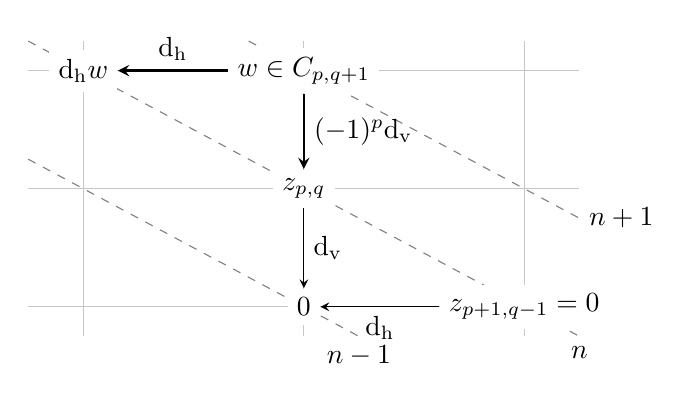
\begin{tikzpicture}[x=2.8cm,y=1.5cm,>=stealth]
\draw[gray!45,step=1] (-1.25,-1.25) grid (1.25,1.25);
\draw[dashed,gray] (-1.25,0.25)--(0.25,-1.25);
\draw[dashed,gray] (-1.25,1.25)--(1.25,-1.25);
\draw[dashed,gray] (-0.25,1.25)--(1.25,-0.25);
\node[fill=white] (w) at (0,1) {\(w\in C_{p,q+1}\)};
\node[fill=white] (z) at (0,0) {\(z_{p,q}\)};
\node[fill=white] (h) at (-1,1) {\(\mathrm d_{\mathrm h}w\)};
\node[fill=white] (v) at (0,-1) {\(0\)};
\node[fill=white] (r) at (1,-1) {\(z_{p+1,q-1}=0\)};
\draw[->,thick] (w)--(z) node[midway,right] {\((-1)^p\mathrm d_{\mathrm v}\)};
\draw[->,thick] (w)--(h) node[midway,above] {\(\mathrm d_{\mathrm h}\)};
\draw[->] (z)--(v) node[midway,right] {\(\mathrm d_{\mathrm v}\)};
\draw[->] (r)--(v) node[midway,below] {\(\mathrm d_{\mathrm h}\)};
\node[below] at (0.25,-1.25) {\(n-1\)};
\node[below] at (1.25,-1.25) {\(n\)};
\node[right] at (1.25,-0.25) {\(n+1\)};
\end{tikzpicture}
\end{center}
图中右侧分量为零，表示刚才选取最大横指标所排除的贡献。减去 \(\mathrm dw\) 消去 \(z_{p,q}\)，只在 \(C_{p-1,q+1}\) 留下修正 \(-\mathrm d_{\mathrm h}w\)，不会产生更右的分量。

于是 \(z-\mathrm{d}w\) 仍为圈，横指标 \(p\) 的分量已经消失，而新产生的分量至多位于横指标 \(p-1\)。第一象限中横指标不小于零，且次数 \(n\) 上只有 \(0\le p\le n\) 的位置；不断降低最大横指标，有限步后得到零。因此原圈是这些 \(w\) 的和的边界。横行正合时，交换两个指标；在 \(C_{p,q}\) 上乘符号 \((-1)^{pq}\)，给出交换前后两个全复形的同构，于是归入刚才的情形。
\end{proof}

\begin{lemma}[Tor 的平衡计算]\label{b3:lem:tor-balanced-computation}
设 \(R\) 为交换环，\(P_\bullet\rightarrow N\rightarrow0\) 与 \(Q_\bullet\rightarrow M\rightarrow0\) 为 \(R\) 模的自由消解。对每个整数 \(i\ge0\)，两条增广映射诱导自然同构
\[
H_i(P\otimes_RM)
\xleftarrow{\ \sim\ }H_i(\operatorname{Tot}(P\otimes_RQ))
\xrightarrow{\ \sim\ }H_i(N\otimes_RQ).
\]
因而用任一变量的自由消解都可计算 Tor，并有自然同构
\[
\operatorname{Tor}_i^R(N,M)\cong\operatorname{Tor}_i^R(M,N).
\]
\end{lemma}
\begin{proof}
取 \(C_{p,q}=P_p\otimes_RQ_q\)，水平、竖直微分分别为 \(\mathrm{d}_P\otimes1\)、\(1\otimes\mathrm{d}_Q\)。在纯张量上，全微分为
\[
\mathrm{d}(u\otimes v)=\mathrm{d}_Pu\otimes v+(-1)^p u\otimes\mathrm{d}_Qv.
\]
由 \(Q_0\twoheadrightarrow M\) 得到逐项满射
\(\alpha:\operatorname{Tot}(C)\rightarrow P\otimes_RM\)：它在 \(q=0\) 的分量上为增广映射，在 \(q>0\) 的分量上为零。这个映射把每条竖直消解在底端压到 \(P_p\otimes_RM\)。要保留被它删去的部分，核在 \(q>0\) 的位置仍取全部分量，底行则必须换成增广映射的核，而不能仍取整个 \(P_p\otimes_RQ_0\)。因此核是下面双复形 \(D\) 的全复形：
\[
D_{p,q}=P_p\otimes_RQ_q\quad(q>0),
\qquad
D_{p,0}=\ker(P_p\otimes_RQ_0\longrightarrow P_p\otimes_RM).
\]
水平微分与增广映射交换，所以保持底行的核；竖直微分从 \(q=1\) 出发时也落入这个核，故 \(D\) 确实是双复形。因为 \(P_p\) 自由，\(Q\) 的增广正合列张量 \(P_p\) 后仍正合，特别地从 \(P_p\otimes_RQ_1\) 到该底行核的映射满射。因此 \(D\) 的每条竖列正合，\cref{b3:lem:first-quadrant-column-exact}说明 \(\ker\alpha=\operatorname{Tot}(D)\) 正合。

这使 \(\alpha\) 在同调上成为同构：给 \(P\otimes_RM\) 中的圈任取提升，其微分落在核中；利用核的正合性减去适当核元素，便得到圈的提升。若全复形中的圈映为边界，先提升产生该边界的元素并减去它的微分，余下的圈落在核中，又是核中的边界。这分别证明满射与单射。

用 \(P_0\twoheadrightarrow N\) 得到另一条逐项满射
\(\beta:\operatorname{Tot}(C)\rightarrow N\otimes_RQ\)。此时将最左列 \(P_0\otimes_RQ_q\) 换成它到 \(N\otimes_RQ_q\) 的核，正是同样的截取。因每个 \(Q_q\) 自由，其核的每条横行正合，同一引理证明 \(\beta\) 也诱导同调同构。这就得到平衡计算。交换张量因子的映射
\[
u\otimes v\longmapsto(-1)^{pq}v\otimes u
\qquad(u\in P_p,\ v\in Q_q)
\]
保持全微分，并交换两条增广映射；于是得到 Tor 的对称性。对 \(N,M\) 的同态选比较链映射后，这些张量映射与增广映射交换；结合\cref{b3:cor:tor-well-defined-functor}的选择无关性，所述同构对两个变量都是自然的。因此以后选取较易消解的变量，并不会改变 Tor 模及其上由同态诱导的映射。
\end{proof}

\subsection{长正合列与 Koszul 计算}
\label{b3:subsec:1505:04}

\begin{lemma}\label{b3:lem:tor-basic-properties}
设 \(R\) 为交换环，\(N,M\) 为 \(R\) 模。Tor 具有自然同构
\[
\operatorname{Tor}_i^R(N,M)\cong\operatorname{Tor}_i^R(M,N)
\qquad(i\ge0),
\]
并在任一变量的短正合列上给出自然长正合列。例如，对 \(R\) 模短正合列
\(0\rightarrow M'\rightarrow M\rightarrow M''\rightarrow0\)，对整数 \(i\ge1\) 有
\[
\begin{aligned}
\cdots&\longrightarrow\operatorname{Tor}_i^R(N,M')
\longrightarrow\operatorname{Tor}_i^R(N,M)
\longrightarrow\operatorname{Tor}_i^R(N,M'')\\
&\xrightarrow{\delta}\operatorname{Tor}_{i-1}^R(N,M')
\longrightarrow\cdots\longrightarrow\operatorname{Tor}_1^R(N,M'')\\
&\xrightarrow{\delta}N\otimes_RM'
\longrightarrow N\otimes_RM
\longrightarrow N\otimes_RM''\longrightarrow0.
\end{aligned}
\]
若 \(a\in R\) 满足 \(aN=0\) 或 \(aM=0\)，则 \(a\operatorname{Tor}_i^R(N,M)=0\) 对每个 \(i\ge0\) 成立。若其中一个模平坦，则所有 \(i>0\) 的 Tor 为零。

对固定的 \(R\) 模 \(M\)，还有等价关系
\[
\begin{aligned}
M\;\text{平坦}
&\iff \operatorname{Tor}_1^R(N,M)=0
   \quad\text{对每个}\;R\;\text{模}\;N\\
&\iff \operatorname{Tor}_1^R(R/I,M)=0
   \quad\text{对每个理想}\;I\subseteq R.
\end{aligned}
\]
对任意理想 \(I,J\subseteq R\)，有自然同构
\[
\operatorname{Tor}_1^R(R/I,R/J)\cong(I\cap J)/IJ.
\]
\end{lemma}
\begin{proof}
对称性已由\cref{b3:lem:tor-balanced-computation}证明。固定 \(N\) 的自由消解 \(P\)，其各项自由，故给定短正合列张量 \(P_i\) 后仍正合，得到复形的逐项短正合列
\[
0\longrightarrow C'\xrightarrow{j}C\xrightarrow{q}C''\longrightarrow0,
\qquad
C'=P\otimes_RM',\quad C=P\otimes_RM,\quad C''=P\otimes_RM''.
\]
商复形中的圈任取一个提升后未必还是圈，但其微分误差必落在子复形中，并给出低一阶的圈；连接映射记录的就是这个误差的同调类。具体地，对 \(C''_i\) 中的圈 \(z''\)，取 \(C_i\) 中的提升 \(z\)。因 \(q(\mathrm{d}z)=0\)，存在唯一 \(z'\in C'_{i-1}\) 使 \(jz'=\mathrm{d}z\)。又由 \(j\) 单射及 \(j\mathrm{d}z'=\mathrm{d}^2z=0\)，有 \(\mathrm{d}z'=0\)。规定 \(\delta[z'']=[z']\)。改变提升只使 \(z'\) 增加一个边界；若 \(z''\) 增加边界 \(\mathrm{d}w''\)，提升 \(w''\) 并将其微分加到 \(z\) 上，\(z'\) 不变。因此连接映射良定义。

正合性在三类位置上直接核验。若 \(C\) 中的圈投到 \(C''\) 的边界，提升产生该边界的元素并减去其微分，便得到来自 \(C'\) 的圈。若 \(\delta[z'']=0\)，写 \(z'=\mathrm{d}v'\)，则 \(z-jv'\) 是 \(z''\) 的圈提升。若 \(C'\) 中的圈 \(z'\) 在 \(C\) 中成为边界 \(jz'=\mathrm{d}w\)，则 \(qw\) 为圈，且 \(\delta[qw]=[z']\)。这证明长列中各处正合；次数零的识别由\cref{b3:cor:tor-well-defined-functor}给出，末尾的满射由张量积右正合性得到。特别地，最低一段中 \(\delta\) 的像正是 \(N\otimes_RM'\to N\otimes_RM\) 的核，补回了张量后可能失去的单射信息。圈提升的构造与复形映射相容，故长列自然。第一变量的短正合列由平衡性得到相同结论。

若 \(aN=0\)，则 \(P\) 上的乘法 \(a\) 与零链映射都提升 \(N\) 上的零同态。\cref{b3:lem:free-resolution-comparison}给出它们之间的链同伦，张量 \(M\) 后仍成立，所以乘法 \(a\) 在同调上为零。若 \(aM=0\)，乘法 \(a\) 在 \(P\otimes_RM\) 上已为零。

若 \(M\) 平坦，令 \(Z_{-1}=N\)、\(Z_i=\ker\mathrm{d}_i\) 对 \(i\ge1\)，并令 \(Z_0=\ker(P_0\rightarrow N)\)。自由消解的正合性给出
\[
0\longrightarrow Z_i\longrightarrow P_i\longrightarrow Z_{i-1}\longrightarrow0
\qquad(i\ge0).
\]
每条短列张量 \(M\) 后仍正合，所以 \(P\otimes_RM\) 的正次数同调为零。若 \(N\) 平坦，交换两个变量即可。

反过来，若 \(\operatorname{Tor}_1^R(N,M)=0\) 对每个 \(N\) 成立，对任意短正合列 \(0\to U\to V\to W\to0\) 在第一变量中使用刚证的长列。\(\operatorname{Tor}_1^R(W,M)=0\) 使 \(U\otimes_RM\to V\otimes_RM\) 的核为零，故 \(M\) 平坦。更少的测试对象已经足够：对任意理想 \(I\)，因 \(R\) 自由，由 \(0\to I\to R\to R/I\to0\) 得到
\[
0\longrightarrow\operatorname{Tor}_1^R(R/I,M)
\longrightarrow I\otimes_RM\longrightarrow M.
\]
这里最后一个映射是 \(a\otimes m\mapsto am\)，所以 \(\operatorname{Tor}_1^R(R/I,M)\) 自然识别为理想张量判据中的核。若这些 Tor 对所有 \(I\) 都为零，\cref{b3:thm:ideal-flatness-criterion}便给出平坦性；前面已经证明平坦性使全部正次 Tor 消失，这完成所述等价关系。

在同一短列中取 \(M=R/J\)。映射
\(I\otimes_R(R/J)\to I/JI\)、\(a\otimes\bar r\mapsto ra+JI\)，与 \(a+JI\mapsto a\otimes\bar1\) 互逆；后一个映射良定义，因为 \(j\in J\) 时有 \(ja\otimes\bar1=a\otimes\bar j=0\)。因而得到
\[
0\longrightarrow\operatorname{Tor}_1^R(R/I,R/J)
\longrightarrow I/JI\longrightarrow R/J,
\qquad a+JI\longmapsto a+J.
\]
最后一个映射的核由恰好属于 \(J\) 的 \(a\in I\) 给出，即 \((I\cap J)/IJ\)。这证明交理想公式，且所有映射都来自包含、取商和张量积，因而同构自然。交 \(I\cap J\) 中未被乘积 \(IJ\) 消去的部分，由此成为一次 Tor 的具体表达。
\end{proof}

一般定义中的自由消解可以任意选择；当给定序列在 \(R\) 上正则时，前面构造的 Koszul 复形已经是 \(R/I\) 的自由消解，所以抽象的 Tor 可以直接用它的微分计算。

\begin{corollary}\label{b3:cor:koszul-tor}
设 \(R\) 为交换环，\(r\ge0\) 为整数，\(x=(x_1,\ldots,x_r)\) 是 \(R\) 上的正则序列，\(I=(x_1,\ldots,x_r)\)。对任意 \(R\) 模 \(M\) 与整数 \(i\ge0\)，有
\[
\operatorname{Tor}_i^R(R/I,M)\cong H_i(x;M).
\]
若 \(IM=0\)，则 \(\operatorname{Tor}_i^R(R/I,M)\cong M^{\binom ri}\) 对 \(0\le i\le r\) 成立，\(i>r\) 时为零。

特别地，设 \(k\) 为域，\(d\ge0\) 为整数，令
\[
R=k[X_1,\ldots,X_d]_{(X_1,\ldots,X_d)},
\qquad \mathfrak m=(X_1,\ldots,X_d)R,
\]
其剩余域 \(R/\mathfrak m\) 自然识别为 \(k\)。则对 \(0\le i\le d\)，有
\[
\operatorname{Tor}_i^R(k,k)\cong\bigwedge_k^ik^d,
\qquad
\dim_k\operatorname{Tor}_i^R(k,k)=\binom di;
\]
对 \(i>d\)，有 \(\operatorname{Tor}_i^R(k,k)=0\)。
\end{corollary}
\begin{proof}
用\cref{b3:thm:koszul-regular-resolution}给出的自由消解计算 Tor。若 \(IM=0\)，张量后的每个微分项 \(x_jm\) 都为零，同调就是复形本身各项，即所述的有限直和。

在局部多项式模型中，模掉 \(X_1,\ldots,X_{j-1}\) 后得到整环
\(k[X_j,\ldots,X_d]_{(X_j,\ldots,X_d)}\)，其中 \(X_j\) 非零，所以乘 \(X_j\) 单射。最终商为非零域 \(k\)，故变量序列是 \(R\) 正则序列；\(d=0\) 时则是空序列。其 Koszul 自由消解张量 \(k\) 后，所有 \(X_j\) 都作用为零，于是微分全为零，第 \(i\) 项按递增指标楔积基识别为 \(\bigwedge_k^ik^d\)。这组基的数目为 \(\binom di\)，且次数超过 \(d\) 时复形本身已经为零，得到所述同调与维数。
\end{proof}

在这个局部多项式模型中，\(k^d\) 通过标准基送到 \(X_j+\mathfrak m^2\)，识别为余切空间 \(\mathfrak m/\mathfrak m^2\)。因此一次 Tor 保留这些一次函数类，高次 Tor 则给出它们的外幂；由\cref{b3:prop:tangent-cotangent-rational}，切空间是这个余切空间的 \(k\) 线性对偶。


\begin{chaptersummary}
正则序列的条件施加在逐次商上，不能只在原环中检验各元素。局部环上的有限生成模中，Nakayama 引理保证商不消失，Krull 交定理则使相邻元素可以交换次序。

\ProseParagraphBreak
Koszul 微分由删去外积因子和交替符号构成；微分平方为零来自同一对因子的两种删法相消。加进一个元素，相当于把原复形与其移位组合起来，其连接映射就是该元素的乘法。这条正合列既证明正则序列给出消解，也把局部逆命题归结为有限生成同调模上的 Nakayama 引理。

\ProseParagraphBreak
自由消解张量后出现的同调是 Tor。消解之间的比较映射在链同伦意义下唯一，因而这些同调不依赖消解的选择，并具有两变量的函子性。一个正则序列的 Koszul 消解在被该序列零化的模上变成零微分复形，因而能直接计算 Tor；商环有多个不可约分量或非零幂零元，并不自动破坏原序列的正则性。
\end{chaptersummary}

\BookExercises

\begin{exercise}\label{b3:ex:15-module-choice}
设 \(k\) 为域，\(R=k[X,Y]\)。分别判断 \(X\) 在 \(R/(Y)\)、\(R/(X)\)、\(R/(XY)\) 上是否为非零因子；在成立时，判断单元素序列 \(X\) 是否正则。
\end{exercise}
\begin{solution}
第一模同构于 \(k[X]\)，乘 \(X\) 单射且商为 \(k\)，故序列正则。第二模中 \(X\) 作用为零而模非零，故不是非零因子。第三模中非零的 \(\bar Y\) 被 \(X\) 零化，也不成立。
\end{solution}

\begin{exercise}\label{b3:ex:15-powers}
设 \(R\) 为交换环，\(M\ne0\) 为 \(R\) 模，\(x,y\) 是 \(M\) 正则序列。证明对任意正整数 \(a,b\)，\(x^a,y^b\) 仍为 \(M\) 正则序列。
\end{exercise}
\begin{solution}
\(x^a\) 显然单射。证明 \(y\) 在 \(M/x^aM\) 上单射：若 \(ym=x^an\)，模掉 \(xM\) 得 \(m=xm_1\)，约去 \(x\) 后有 \(ym_1=x^{a-1}n\)，反复进行得 \(m\in x^aM\)。所以 \(y^b\) 也在该商上单射。末端商 \(M/(x^a,y^b)M\) 满射到非零的 \(M/(x,y)M\)，因而非零。
\end{solution}

\begin{exercise}\label{b3:ex:15-order-localization}
设 \(k\) 为域，\(R=k[X,Y]\)，\(M=R\oplus R/(X-1,Y)\)。在极大理想 \((X,Y)\) 处局部化，解释为何原来不正则的次序 \(Y,X\) 在 \(M_{(X,Y)}\) 上变成正则。
\end{exercise}
\begin{solution}
\(X-1\) 在该局部环中是单位，故第二直和项局部化为零，剩下 \(k[X,Y]_{(X,Y)}\)。先模掉 \(Y\) 得 \(k[X]_{(X)}\)，其中 \(X\) 为非零因子，末端商为 \(k\)，所以 \(Y,X\) 正则。原来的乘法核全部位于被这次局部化删去的支集部分。
\end{solution}

\begin{exercise}\label{b3:ex:15-flat-not-faithful}
设 \(k\) 为域，取 \(R=k[T]\times k[T]\)，\(S=k[T]\) 为投影到第一因子的 \(R\) 代数，\(x=(T,0)\)。证明 \(S\) 平坦但不忠实，并说明 \(x\) 在 \(S\) 上正则不能推出它在 \(R\) 上正则。
\end{exercise}
\begin{solution}
\(S\) 作为 \(R\) 模是幂等元 \((1,0)\) 给出的直和项，故投射、从而平坦。非零模 \(0\times k[T]\) 与 \(S\) 张量为零，所以不忠实。\(x\) 在 \(S\) 上就是 \(T\)，乘法单射且商为 \(k\)；在 \(R\) 上却零化非零元 \((0,1)\)。
\end{solution}

\begin{exercise}\label{b3:ex:15-koszul-localize-unit}
设 \(k\) 为域，\(R=k[X,Y]\)，\(M=R_X\oplus R_Y\)。计算 \(H_i(X,Y;M)\)，并证明虽然 \(I=(X,Y)\) 是 \(R\) 的真理想，却有 \(IM=M\)。判断该序列是否 \(M\) 正则，并说明 \(M_{(X,Y)}\) 是否为非零有限生成模。
\end{exercise}
\begin{solution}
复形按两个系数模分成直和。在 \(R_X\) 上用 \(X^{-1}e_1\wedge(-)\)，在 \(R_Y\) 上用 \(Y^{-1}e_2\wedge(-)\)，所得同伦均满足 \(\mathrm{d}h+h\mathrm{d}=\operatorname{id}\)，所以全部同调为零。又因 \(XR_X=R_X\)、\(YR_Y=R_Y\)，有 \(IM=M\)。末端商为零，序列不满足本章正则序列的非退化条件。

\ProseParagraphBreak
在 \(\mathfrak m=(X,Y)\) 处，\(M_{\mathfrak m}=R_{\mathfrak m}[X^{-1}]\oplus R_{\mathfrak m}[Y^{-1}]\) 非零，因为这两个局部化都嵌入 \(R\) 的分式域。若它有限生成，由 \(\mathfrak mM_{\mathfrak m}=M_{\mathfrak m}\) 和 Nakayama 引理便得 \(M_{\mathfrak m}=0\)，矛盾。因此它不是有限生成模，不能套用局部有限生成模的 Koszul 正则性判据。
\end{solution}

\begin{exercise}\label{b3:ex:15-three-matrices}
对任意交换环 \(R\) 中的 \(x,y,z\)，在二次外幂中采用基 \(e_1\wedge e_2,e_1\wedge e_3,e_2\wedge e_3\)，写出 \(K_\bullet(x,y,z;R)\) 的三个微分矩阵，并计算相邻矩阵乘积。
\end{exercise}
\begin{solution}
三个矩阵依次为
\[
\mathrm{d}_1=(x\ \ y\ \ z),\qquad
\mathrm{d}_2=\begin{pmatrix}-y&-z&0\\x&0&-z\\0&x&y\end{pmatrix},
\qquad \mathrm{d}_3=\begin{pmatrix}z\\-y\\x\end{pmatrix}.
\]
\(\mathrm{d}_1\mathrm{d}_2\) 的分量为 \(-xy+yx,-xz+zx,-yz+zy\)，均为零；\(\mathrm{d}_2\mathrm{d}_3\) 的分量为 \(-yz+zy,xz-zx,-xy+yx\)，也均为零。这里只用交换性，特征二时两项仍相消。
\end{solution}

\begin{exercise}\label{b3:ex:15-generator-operation}
设 \(R\) 为交换环，\(x,y,a\in R\)，\(M\ne0\) 为 \(R\) 模。构造 \(K_\bullet(x,y+ax;R)\) 与 \(K_\bullet(x,y;R)\) 的同构，并说明替换 \(y\) 为 \(y+ax\) 是否改变 \(x,y\) 在 \(M\) 上的正则性。
\end{exercise}
\begin{solution}
把新一次基 \(f_1,f_2\) 分别送到 \(e_1,e_2+ae_1\)。其微分分别为 \(x,y+ax\)，且基变换矩阵行列式为一，故在全部外幂上给出可逆链映射。张量 \(M\) 后仍为同构。正则性可直接由定义判断：第一步仍是乘 \(x\)，而在 \(M/xM\) 上有
\[
(y+ax)m\equiv ym\pmod{xM},
\qquad (x,y+ax)M=(x,y)M.
\]
因此第二步的乘法映射及末端商都没有改变，\(x,y\) 与 \(x,y+ax\) 的正则性等价。
\end{solution}

\begin{exercise}\label{b3:ex:15-repeated-equation}
设 \(R\) 为整环，\(0\ne x\in R\) 为非单位元。计算 \(K_\bullet(x,x,x;R)\) 的全部同调，并写出次数一、二同调的生成圈。
\end{exercise}
\begin{solution}
换基为 \(g_1=e_1\)、\(g_2=e_2-e_1\)、\(g_3=e_3-e_1\)。这是行列式为一的整数换基，且 \(\mathrm{d}g_1=x\)、\(\mathrm{d}g_2=\mathrm{d}g_3=0\)。因此复形分成四个由 \(1,g_2,g_3,g_2\wedge g_3\) 标记的两项复形，微分在每个非零配对中都是乘 \(x\)（至多相差符号）。乘 \(x\) 单射，故
\[
H_0=R/(x),\qquad H_1=(R/(x))^2,\qquad H_2=R/(x),\qquad H_3=0.
\]
次数一的两组生成圈为 \(g_2,g_3\)，次数二的生成圈为 \(g_2\wedge g_3\)。这些类的系数均模掉 \((x)\)；三次同调为零来自乘 \(x\) 的单射性。
\end{solution}

\begin{exercise}\label{b3:ex:15-dual-numbers}
设 \(k\) 为域，令 \(R=k[\varepsilon]/(\varepsilon^2)\)。分别计算 \(K_\bullet(\varepsilon;R)\) 与 \(K_\bullet(\varepsilon;R/(\varepsilon))\) 的同调，并比较原因。
\end{exercise}
\begin{solution}
第一复形中乘法核为 \((\varepsilon)\cong k\)，余核也为 \(k\)。第二复形的微分为零，所以两处同调都为 \(k\)。前者的非正合性来自环中真实的零因子，后者则因为张量系数模使乘法完全消失。
\end{solution}

\begin{exercise}\label{b3:ex:15-crossing-homology}
设 \(k\) 为域，\(R=k[X,Y]/(XY)\)，\(\bar X,\bar Y\) 为变量的余类。计算 \(H_i(\bar X,\bar Y;R)\)。
\end{exercise}
\begin{solution}
把 \(R\) 写成常数项相同的多项式配对，可知 \(\operatorname{Ann}(\bar X)=(\bar Y)\)、\(\operatorname{Ann}(\bar Y)=(\bar X)\)，两理想交为零。一次圈恰为 \((\bar Ya,\bar Xb)\)，边界为 \((-\bar Yc,\bar Xc)\)。取 \(c=1\) 得
\[
[(0,\bar X)]=[(\bar Y,0)]\quad\text{于 }H_1.
\]
这一类被 \(\bar X,\bar Y\) 零化：乘 \(\bar X\) 直接得零，乘 \(\bar Y\) 则得到边界 \((\bar Y^2,0)=\mathrm{d}_2(-\bar Y)\)。同样，\(\bar Y,\bar X\) 的二次及更高次幂给出的圈都是边界，所以任意圈都化成该类的 \(k\) 倍。这个类非零，否则须有 \(c\) 同时满足 \(-\bar Yc=\bar Y\)、\(\bar Xc=0\)，前式要求其常数项为 \(-1\)，后式要求为零，矛盾。因此 \(H_1\cong k\)，最高同调为上述零化子之交，故 \(H_2=0\)，而 \(H_0=k\)。
\end{solution}

\begin{exercise}\label{b3:ex:15-triangular-complete-intersection}
设 \(k\) 为域，\(R=k[X,Y,Z]\)。证明 \(Y-X^2,Z-Y^2,Z\) 是正则序列，计算末端商的 \(k\) 维数，并写出自由消解各项的秩。
\end{exercise}
\begin{solution}
依次前两次商为 \(k[X,Z]\)、\(k[X]\)，所以前两步乘法都是整环中非零元的乘法。此时 \(Z\) 的像为 \(X^4\)，仍为非零因子，末端商为 \(k[X]/(X^4)\)，维数为四。三元 Koszul 消解从次数零至三的秩依次为 \(1,3,3,1\)。
\end{solution}

\begin{exercise}\label{b3:ex:15-component-section}
设 \(k\) 为域，令 \(A=k[U,V]/(UV)\)，仍以 \(U,V\) 记变量的余类。对 \(a,b\in k\)，判断 \(aU+bV\) 何时在 \(A\) 上为非零因子，并在成立时求其商环。
\end{exercise}
\begin{solution}
若 \(a=0\)，则该元素被非零的 \(U\) 零化；\(b=0\) 同理。若 \(a,b\ne0\)，用常数项相同的配对模型，乘法分别为乘 \(aU,bV\)，故单射。在商中 \(V=-ab^{-1}U\)，关系 \(UV=0\) 变成 \(U^2=0\)，所以商环为 \(k[U]/(U^2)\)。
\end{solution}

\begin{exercise}\label{b3:ex:15-tor-integers}
设 \(m,n\) 为正整数，计算 \(\operatorname{Tor}_i^{\mathbb Z}(\mathbb Z/m,\mathbb Z/n)\) 对所有 \(i\ge0\) 的值。
\end{exercise}
\begin{solution}
用 \(\mathbb Z\xrightarrow{m}\mathbb Z\) 的自由消解。张量后为 \(\mathbb Z/n\xrightarrow{m}\mathbb Z/n\)。若 \(d=\gcd(m,n)\)，其核由 \(n/d\) 的余类生成，阶为 \(d\)，余核也为 \(\mathbb Z/d\)。因此次数零、一均为 \(\mathbb Z/d\)，其余次数为零。
\end{solution}

\begin{exercise}\label{b3:ex:15-intersection-tor}
设 \(k\) 为域，\(R=k[X,Y,Z]\)，\(I=(X,Y)\)、\(J=(Y,Z)\)。计算 \(\operatorname{Tor}_i^R(R/I,R/J)\) 对所有 \(i\ge0\) 的值；再计算 \((I\cap J)/IJ\)，与次数一的答案比较。
\end{exercise}
\begin{solution}
\(X,Y\) 正则，其 Koszul 消解张量 \(R/J=k[X]\) 后成为 \(K_\bullet(X,0;k[X])\)。乘 \(X\) 单射，因此次数零、一同调均为 \(k\)，其余同调为零。

\ProseParagraphBreak
模掉 \(Y\) 后，\(k[X,Z]\) 中 \((X)\cap(Z)=(XZ)\)，故
\[
I\cap J=(Y,XZ),\qquad IJ=(XY,XZ,Y^2,YZ).
\]
商由 \(Y\) 的类生成；它被 \(X,Y,Z\) 零化而不为零，因为 \(Y\notin IJ\)。这个商因而同构于 \(k\)，与正文的交理想公式及上述 \(\operatorname{Tor}_1\) 计算一致。
\end{solution}

\begin{exercise}\label{b3:ex:15-residue-tor}
设 \(k\) 为域，\(R=k[X,Y]_{(X,Y)}\)，\(a,b\ge2\) 为整数，\(A=R/(X^a,Y^b)\)。计算 \(\operatorname{Tor}_i^R(k,A)\)，并在 \(K_\bullet(X,Y;A)\) 中写出同调的 \(k\) 基。
\end{exercise}
\begin{solution}
\(X^a,Y^b\) 在多项式环中正则，局部化后末端商仍非零，故也是 \(R\) 正则序列。其 Koszul 消解张量 \(k\) 后微分为零，得到 \(\operatorname{Tor}_i^R(A,k)\) 在次数零、一、二的维数分别为 \(1,2,1\)，其余为零。由平衡性，\(\operatorname{Tor}_i^R(k,A)\) 同样如此。

\ProseParagraphBreak
\(A\) 同构于 \(k[X,Y]/(X^a,Y^b)\)：在后一个环中，常数项非零的元素都是单位，因为其余部分幂零。它有基 \(X^iY^j\)（\(0\le i<a,0\le j<b\)）。在 \(K_\bullet(X,Y;A)\) 中，\(H_0\) 的基为 \([1]\)，\(H_1\) 的候选基为
\[
[X^{a-1}e_1],\qquad [Y^{b-1}e_2],
\]
\(H_2\) 的候选基为 \([X^{a-1}Y^{b-1}e_1\wedge e_2]\)。它们都是圈。若一次圈的上述 \(k\) 线性组合是边界 \((-Yc,Xc)\)，第一分量模掉 \(Y\)、第二分量模掉 \(X\)，分别迫使两个系数为零，所以两类独立。次数二的圈非零且无三次边界。结合已算出的同调维数，这些类分别构成所需的基。
\end{solution}

\begin{exercise}\label{b3:ex:15-zero-generator-splitting}
设 \(R\) 为交换环，\(M\) 为 \(R\) 模，\(r\ge0\) 为整数，\(x=(x_1,\ldots,x_r)\in R^r\)。证明
\[
H_i(x,0;M)\cong H_i(x;M)\oplus H_{i-1}(x;M),
\]
并由此计算 \(r\) 个零元素在 \(M\) 上的 Koszul 同调。
\end{exercise}
\begin{solution}
新增元素为零时，分解 \(K_i(x,0;M)=K_i(x;M)\oplus K_{i-1}(x;M)\) 的微分是 \((a,b)\mapsto(\mathrm{d}a,-\mathrm{d}b)\)，两个分量不混合，故同调分裂如式。从空序列的唯一同调 \(M\) 开始反复应用，得到 \(H_i(0,\ldots,0;M)\cong M^{\binom ri}\)，超出 \(0\le i\le r\) 的次数为零。
\end{solution}

\begin{exercise}\label{b3:ex:15-infinite-module-caution}
设 \(R\) 为离散赋值环，统一化元为 \(\pi\)，分式域为 \(K\)。计算 \(K_\bullet(\pi;K)\) 的同调，说明为何不能由次数一同调为零断言 \(\pi\) 是本章意义的 \(K\) 正则序列。
\end{exercise}
\begin{solution}
\(\pi:K\rightarrow K\) 是同构，所以两处同调都为零。末端商 \(K/\pi K=0\)，违反非退化条件。\(K\) 不是有限生成的 \(R\) 模，Nakayama 引理不能用于证明末端商非零，所以局部环上有限生成模的判据不适用。
\end{solution}

\begin{exercise}\label{b3:ex:15-local-detection-obstruction}
设 \(k\) 为域，\(R=k[X,Y,Z]\)。对序列 \(XY,XZ\)，求正次数 Koszul 同调的支集，与 \(V(XY,XZ)\) 比较，并分别判断在素理想 \((X)\)、\((Y,Z)\)、\((Y)\) 处的同调及正则性。
\end{exercise}
\begin{solution}
一次圈满足 \(XYa+XZb=0\)，约去 \(X\) 后得 \(Ya+Zb=0\)，故恰为 \((-Zc,Yc)\)。一次边界为 \(X(-Zc,Yc)\)，而最高微分单射，所以
\[
H_1\cong R/(X),\qquad H_2=0,\qquad
\operatorname{Supp}H_1=V(X)\subsetneq V(X)\cup V(Y,Z)=V(XY,XZ).
\]
在 \((X)\) 处，\(Y,Z\) 都成为单位，两个方程都是 \(X\) 的单位倍，末端商非零且 \(H_1\ne0\)，第二个方程重复了第一个，序列不正则。在 \((Y,Z)\) 处，\(X\) 是单位，序列的正则性等同于 \(Y,Z\) 的正则性；逐次商为整环，末端商是 \(k(X)\)，故序列正则且正次数同调全为零。在 \((Y)\) 处，\(XZ\) 是单位，全部同调与末端商都为零，所以仍不符合本章非退化意义的正则性。
\end{solution}
